\subsection{Zusammensetzung der kosmischen Strahlung} 
Als primäre kosmische Strahlung bezeichnet man die Strahlung, die unmittelbar aus dem All auf die obersten Atmosphärenschichten trifft. Diese Strahlung besteht zu \SI{79}{\percent} aus freien Protonen, ca. \SI{15}{\percent} Heliumkernen und zu einem kleinen Teil aus schweren Atomkernen und Elektronen\cite{pdg}. Die Herkunft der Teilchen ist weitgehend unbekannt. Dies liegt zum einen daran, dass niedrigenergetische Teilchen auf ihrem Weg stark abgelenkt werden können und so isotrop auf die Atmosphäre treffen, also keine bestimmte Richtung haben. Zum anderen gibt es dieses Problem bei hochenergetischen Teilchen zwar nicht, diese sind aber dafür äußerst selten, weshalb es schwer ist, ausreichend Messdaten zu erfassen.  Das spiegelt sich auch im Spektrum der primären kosmischen Strahlung wieder (Abb. \ref{fig:energiespektrum}), bei dem auffällt, dass es sehr breit ist und so z.B. Energien vom LHC im Bereich von \si{\tera\electronvolt} deutlich übertroffen werden. Die Teilchenflussdichte zeigt eine Proportionalität zu $E^{-\lambda}$, nimmt also stark ab.
\begin{figure}[h]
  \centering
  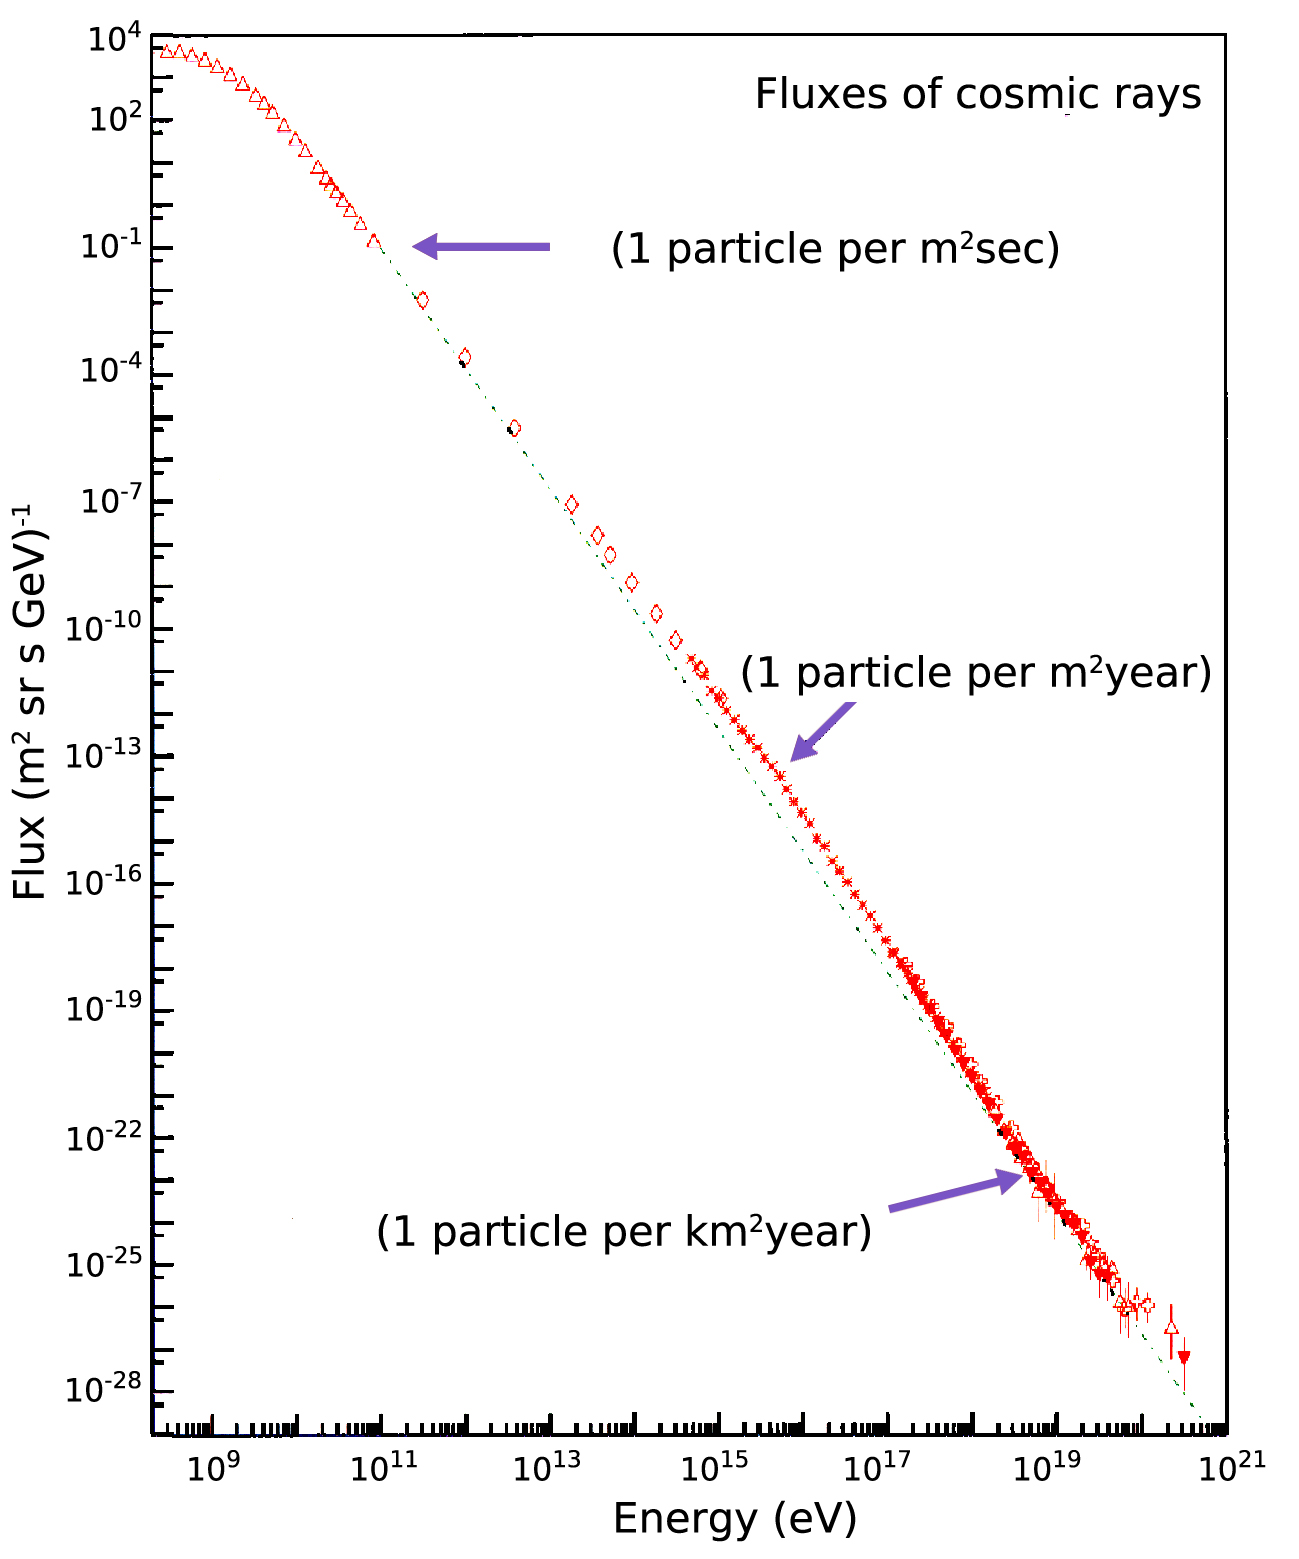
\includegraphics[width=0.5\textwidth]{data/energiespektrum.png}
  \caption{Energiespektrum der primären kosmischen Strahlung, aus \cite{Bietenholz:2013fta}}
  \label{fig:energiespektrum}
\end{figure}  

 Durch Wechselwirkung der Primärteilchen mit der Atmosphäre entsteht die sekundäre kosmische Strahlung (Abb. \ref{fig:schauer}). 

Treffen die Hadronen auf die Stickstoff- und Sauerstoffatome in der Atmosphäre, kommt es zur Spallation, es werden also Neutronen und Protonen aus den Atomen herausgeschlagen. Das ist ein Prozess der starken Wechselwirkung und es entstehen auch weitere Hadronen. Zum größten Teil entstehen dabei Pionen. Pionen\cite{pdg} sind mit einer Ruheenergie von etwa \SI{140}{\mega \electronvolt} die leichtesten Mesonen und sind nicht stabil. Die geladenen Pionen haben eine Lebensdauer von etwa \SI{2.6e-8}{\second} und zerfallen zu über \SI{99.9}{\percent} durch die schwache Wechselwirkung in Myonen
\begin{align*}
  \pi^+ &\rightarrow \mu^+ + \nu_\mu\\
  \pi^- &\rightarrow \mu^- + \bar{\nu}_\mu.
\end{align*}
Die neutralen Pionen zerfallen zu über \SI{98}{\percent} zu zwei Photonen. Dies geschieht durch die elektromagnetische Wechselwirkung und dadurch haben sie eine deutlich kürzere Lebenszeit von etwa \SI{8.5e-17}{\second}.
Myonen\cite{pdg} haben eine Masse von etwa \SI{106}{\mega\electronvolt} und eine mittlere Lebensdauer von ca. \SI{2.2e-6}{\second} und zerfallen dann leptonisch in ein Elektron bzw. Positron
\begin{align*}
  \mu^+ &\rightarrow e^++ \nu_e +\bar{\nu}_\mu\\
  \mu^- &\rightarrow e^-+ \bar{\nu}_e +\nu_\mu.
\end{align*}
Nicht-relativistisch könnten die Myonen die Erdoberfläche kaum erreichen bevor sie zerfallen. Durch die hohe Geschwindigkeit spielt die Zeitdilatation aber eine Rolle und sie können die Erdoberfläche erreichen. In Abbildung \ref{fig:fluss} sind die Teilchenflüsse in Abhängigkeit der atmosphärischen Tiefe zu sehen. Neutrinos sind aufgrund ihrer geringen Wechselwirkung schwer nachzuweisen und somit sind die Myonen ein guter Kandidat zur Untersuchung der Höhenstrahlung.   

\begin{figure}[h]
  \centering
  \begin{subfigure}[h]{0.5\textwidth}
    \centering
    \begin{tikzpicture}[scale=0.8]
      \draw (4,0)--(3.5,-1.5);
      \draw(3.5,-1.5)--(6,-3);
      \draw (4.7,-1.5) node {$\pi^+$};
      \draw(3.5,-1.5)--(2.5,-4);
      \draw (2.8,-2.5) node {$N$};
      \draw(2.5,-4)--(1.5,-5.4);
      \draw(1.5,-5.4)--(0.5,-6);
      \draw(0.5,-5.6) node {$p$};
      \draw(1.5,-5.4)--(1.6,-6);
      \draw (1.6,-6.3) node {$p$};
      \draw(2.5,-4)--(1.8,-8);
      \draw (2.7,-6) node {$\pi^-$};
      \draw[dashed](1.8,-8)--(2,-11);
      \draw(2.3,-9.5) node {$\bar{\nu}_{\mu}$};
      \draw(1.8,-8)--(1,-11);
      \draw(0.7,-10) node {$\mu^-$};
      \draw(3.5,-1.5)--(1,-2.5);
      \draw(2,-1.8) node {$\pi^0$};
      \draw[decorate, decoration={snake}](1,-2.5)--(0,-3.8);
      \draw(0.4,-2.9) node {$\gamma$};
      \draw[decorate, decoration={snake}](1,-2.5)--(1.5,-4);
      \draw(1.4,-3) node {$\gamma$};
      \draw[dashed](6,-3)--(7.5,-3.5);
      \draw(6.8,-3) node {$\nu_{\mu}$};
      \draw(6,-3)--(5,-7);
      \draw(5.2,-5) node {$\mu^+$};
      \draw(5,-7)--(4,-8);
      \draw(4,-7.5) node {$e^+$};
      \draw[dashed](5,-7)--(6,-11);
      \draw(5.8,-9) node {$\bar{\nu}_{\mu}$};
      \draw[dashed](5,-7)--(4,-11);
      \draw(4.2,-9) node {$\nu_e$};
    \end{tikzpicture}
    \subcaption{Mögliche Schauerbildung}
    \label{fig:schauer}
  \end{subfigure}%
  \begin{subfigure}[h]{0.5\textwidth}
    \centering
  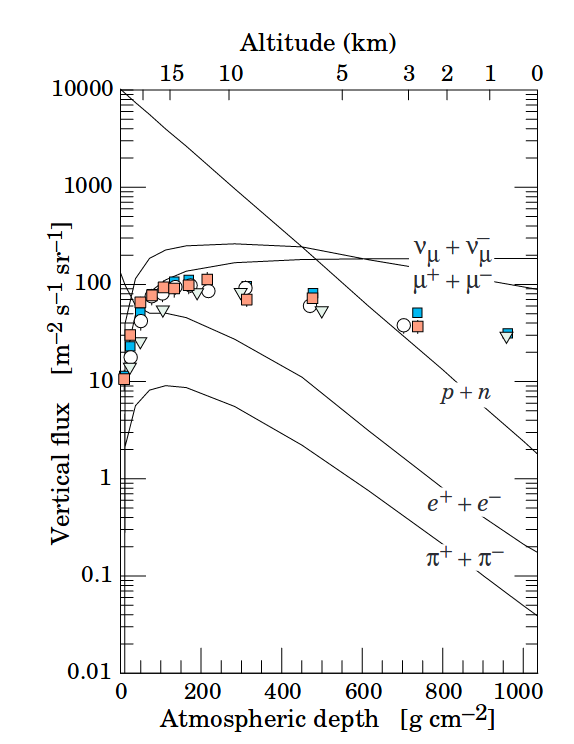
\includegraphics[width=\textwidth]{data/verteilung_sekundaer.png}
  \subcaption{Teilchenzahl in Abhängigkeit der Höhe, aus \cite{pdg}}
  \label{fig:fluss}
  \end{subfigure}
  \caption{Sekundäre Höhenstrahlung}
\end{figure}

\subsection{Energieverlust von Teilchen in Materie}
Geladene Teilchen verlieren beim Durchgang von Materie Energie. Dies geschieht durch die Anregung und Ionisation von Elektronen aus Atomen in der Materie. Die mittlere abgegebene Energie pro Längeneinheit kann durch die Bethe-Formel beschrieben werden\cite{sigmund2014particle}
\begin{align}
  -\left\langle \diff{E}{x} \right\rangle=K\frac{z^2n}{\beta^2}\left(\ln \frac{2m_ec^2\beta^2\gamma^2}{I} -\beta^2 \right).
  \label{eq:bethe}
\end{align}
$m_e$ und $c$ sind dabei die Elektronenmasse und die Lichtgeschwindigkeit. Die Konstante $K$ setzt sich weiter mit der Elementarladung $e$ und der elektrischen Feldkonstante $\epsilon_0$ zusammen zu
\begin{align*}
  K=\frac{e^4}{4\pi \epsilon_0^2m_ec^2}.
\end{align*}
Der einzigen Parameter des einfallenden Teilchens die einfließen sind die Ladungszahl $z$ und die Geschwindigkeit $v$ über
\begin{align*}
  \beta&=v/c\\
  \gamma&=1/\sqrt{1-\beta^2}.
\end{align*}
Die einfließenden Größen des Materials sind die Elektronendichte $n$, die Ladungszahl $Z$ der Atome und die mittlere Anregungsenergie $I$.

In diesem Versuch werden Plastikszintillatoren verwendet. Da das Material nicht genauer spezifiziert ist wird exemplarisch von Polystyrol ausgegangen. Aus \cite{polystyrene} erhält man $I=\SI{68.7}{\electronvolt}$. Aus der angegebenen Dichte und dem Verhältnis von Protonen zu Nukleonen folgt außerdem $n\approx \SI{3.43e29}{\metre^{-3}}$. Der mit Gleichung (\ref{eq:bethe}) resultierende Energieverlust für Myonen ($z=1$) in Abhängigkeit von $\gamma$ ist in Abbildung \ref{fig:bethe} zu sehen.

\begin{figure}[h]
  \centering
  \begin{tikzpicture}
    \draw [->] (0,0)--(0,5.5) node [left] {$-\left\langle \diff{E}{x} \right\rangle/\si{\mega\electronvolt}$};
    \draw [->] (0,0)--(10.5,0) node [right] {$\gamma$};
    \draw[domain=1.23/5:10,smooth,variable=\x,samples=200] plot ({\x},{(17.5/(1-1/(5*\x*5*\x))*(2*ln(121.968*\x*5*sqrt(1-1/(25*\x*\x)))-1+1/(25*\x*\x))-200)/50});
    \foreach \x in {1,10,20,30,40,50}{
       \draw (\x/5,0)--(\x/5,-0.1) node [below] {$\x$};
    }
    \foreach \x in {250,300,350,400,450}{
       \draw (0,\x/50-4)--(-0.1,\x/50-4) node [left] {$\x$};
    }
     \end{tikzpicture}
  \caption{Energieverlust eines Myons in Polystyrol}
  \label{fig:bethe}
\end{figure}
Für dicke Schichten ist der Energieverlust eines durchquerenden Teilchens gaußförmig um den von der Bethe-Bloch-Gleichung vorausgesagten Mittelwert verteilt. Für dünnere Materialien hingegen spielen einzelne Prozesse mit hohem Energieübetrag eine große Rolle und die Gaußverteilung wird zur Landauverteilung. Die Verteilung kann durch
\begin{align}
  p(\Delta E)=\frac{1}{\sqrt{2\pi}}e^{-(\lambda+e^{-\lambda})/2}
  \label{eq:landau}
\end{align}
genähert werden, wobei $\lambda$ durch
\begin{align*}
  \lambda=(\Delta E-\langle \Delta E \rangle)\frac{2 \beta^2}{Kz^2nx}
\end{align*}
gegeben ist\cite{ketzer:vorlesung}. $x$ ist dabei die Dicke des Materials und $\langle \Delta E \rangle$ der mittlere Energieverlust aus der Bethe-Bloch-Gleichung. Exemplarisch wird von Myonen und einem $x=\SI{1}{\cm}$ dicken Szintillator aus Polystyrol ausgegangen. Unter der Annahme, dass die Geschwindigkeit annähernd konstant bleibt gilt
\begin{align*}
  \langle \Delta E \rangle \approx -\left\langle  \diff{E}{x}  \right\rangle x. 
\end{align*}
Für die Geschwindigkeit wird die mittlere Geschwindigkeit von $v\approx 99,4 c$ ($\gamma \approx 9.14$) aus \cite{speed} verwendet. Die aus Gleichung (\ref{eq:landau}) folgende Verteilung mit zusätzlicher Normierung ist in Abbildung \ref{fig:landau} zu sehen.

\begin{figure}[h]
  \centering
  \begin{tikzpicture}
    \draw [->] (-0.5,0)--(-0.5,5.5) node [left] {$p(\Delta E)$};
    \draw [->] (-0.5,0)--(5.5,0) node [right] {$\Delta E/\si{\mega\electronvolt}$};
    \draw[domain=0:5,smooth,variable=\x,samples=200] plot ({\x},{5*1.6487*exp(-(11.29184*(2+0.3*\x-2.30704)+exp(-11.29184*(2+0.3*\x-2.30704)))/2)});
    \foreach \x in {2,2.5,3,3.5}{
       \draw (\x/0.3-2/0.3,0)--(\x/0.3-2/0.3,-0.1) node [below] {$\x$};
    }
    \foreach \x in {0.25,0.5,0.75,1}{
       \draw (-0.5,\x*5)--(-0.6,\x*5) node [left] {$\SI{\x}{}$};
    }
     \end{tikzpicture}
  \caption{Energieverlust eines Myons in Polystyrol}
  \label{fig:landau}
\end{figure}

\subsection{Szintillationszähler}
Ein Szintillator weißt ionisierende Teilchen über den im vorherigen Abschnitt beschriebenen Energieverlust nach. Die Teilchen regen die Atome im Szintillationsmaterial an. Nach einer mittleren Anregungsdauer fällt das Atom zurück in den Grundzustand und emittiert dabei ein Photon der entsprechenden Wellenlänge. Dieses Photon kann nun auch wieder weitere Atome anregen und es kommt zu einer Art Random-Walk. Um diesen zu unterbrechen wird das Szintillationsmaterial schwach mit wellenlängenverschiebenden Molekülen dotiert. Trifft ein Photon auf ein solches wird das Licht zu langwelligerem Licht umgewandelt. Dieses kann nicht vom Szintillator absorbiert werden und kann somit über einen Lichtleiter zu einer Photodiode gelangen. Diese erzeugt eine messbare elektrische Spannung. Der Prozess ist in Abbildung \ref{fig:szintillator} schematisch skizziert.

\begin{figure}[h]
  \centering
  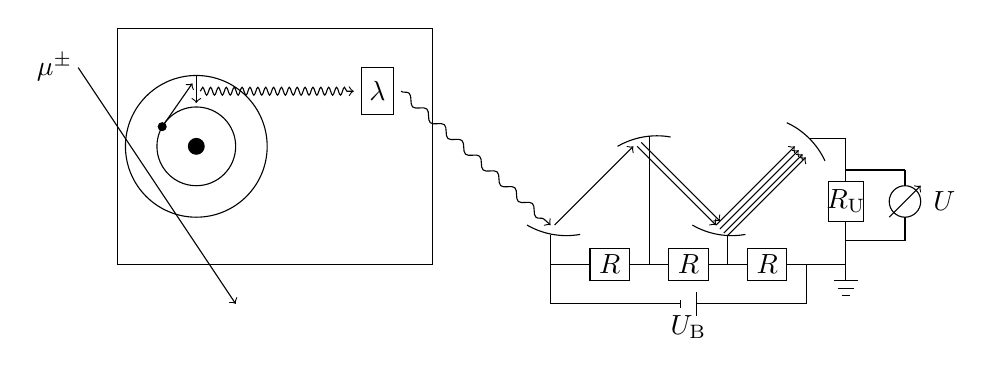
\begin{tikzpicture}[photon1/.style={decorate,decoration={snake, segment length=1mm, amplitude=0.5mm, post length=0.5mm}},photon2/.style={decorate,decoration={snake, segment length=3mm, amplitude=0.5mm, post length=0.5mm}}]
    \draw (0,0) rectangle (4,3);
    \draw [->] (-0.5,2.5)--(1.5,-0.5);
    \draw (-0.8,2.5) node {$\mu^{\pm}$};
    \draw (1,1.5) circle (0.9);
    \draw (1,1.5) circle (0.5);
    \draw [fill=black] (1,1.5) circle (0.1);
    \draw [fill=black] (1-0.5*1.732/2,1.5+1/4) circle (0.05);
    \draw [->] (1-0.5*1.732/2,1.5+1/4)--(0.95,2.3);
    \draw [->] (1,2.4) -- (1,2.05);
    \draw [->,photon1] (1.05,2.2) -- (3,2.2);
    \draw (3.1,1.9) rectangle (3.5,2.5);
    \draw (3.3,2.2) node {$\lambda$};
    \draw [->,photon2] (3.6,2.2)-- (5.5,0.5);
    \draw (5.2,0.5) arc (-120:-80:1);
    \draw [->] (5.55,0.5) -- (6.55,1.5);
    \draw (6.35,1.5) arc (120:80:1);
    \draw [->] (6.6,1.5) -- (7.6,0.5);
    \draw [->] (6.65,1.55) -- (7.65,0.55);
    \draw (7.3,0.5) arc (-120:-80:1);
    \draw [->] (7.65,0.45) -- (8.65,1.45);
    \draw [->] (7.6,0.5) -- (8.6,1.5);
    \draw [->] (7.7,0.4) -- (8.7,1.4);
    \draw [->] (7.74,0.36) -- (8.74,1.36);
    \draw (8.5,1.8) arc (65:25:1);
    \draw (9,0)--(8.5,0);
    \draw (8.75,0)--(8.75,-0.5)--(7.35,-0.5);
    \draw (7.15,-0.5)--(5.5,-0.5)--(5.5,0);
    \draw (8.5,0.2) rectangle (8,-0.2);
    \draw (8.25,0) node {$R$};
    \draw (8,0) -- (7.5,0);
    \draw (7.5,0.2) rectangle (7,-0.2);
    \draw (7.25,0) node {$R$};
    \draw (7,0) -- (6.5,0);
    \draw (7.75,0)--(7.75,0.375);
    \draw (6.75,0)--(6.75,1.635);
    \draw (6.5,0.2) rectangle (6,-0.2);
    \draw (6.25,0) node {$R$};
    \draw (6,0)--(5.5,0)--(5.5,0.375);
    \draw (7.35,-0.65)--(7.35,-0.35);
    \draw (7.15,-0.55)--(7.15,-0.45);
    \draw (7.25,-0.8) node {$U_\mathrm{B}$};
    \draw (9,0)--(9.25,0)--(9.25,0.55);
    \draw (9.03,0.55) rectangle (9.47,1.05);
    \draw (9.25,0.8) node {$R_\mathrm{U}$};
    \draw (9.25,1.05)--(9.25,1.6)--(8.8,1.6);
    \draw (9.25,0)--(9.25,-0.2);
    \draw (9.1,-0.2)--(9.4,-0.2);
    \draw (9.15,-0.3)--(9.35,-0.3);
    \draw (9.2,-0.4)--(9.3,-0.4);
    \draw (9.25,0.3)--(10,0.3);
    \draw (9.25,1.2)--(10,1.2);
    \draw (10,0.8) circle (0.2);
    \draw (10,0.3)--(10,0.6);
    \draw (10,1.2)--(10,1);
    \draw [->] (9.8,0.6)--(10.2,1);
    \draw (10.5,0.8) node {$U$};
  \end{tikzpicture}
  \caption{Signalerzeugung in Szintillator}
  \label{fig:szintillator}
\end{figure} 

\subsection{Diskriminator und Koinzidenzmodul}
Für die Zählung der Myonen aus der kosmischen Strahlung werden die analogen Signale der Szintillatoren in digitale Signale umgewandelt. Dazu werden Diskriminatoren verwendet. Gibt der Szintillator ein Signal über der einstellbaren Schwellenspannung $\delta U$ an den Diskriminator gibt dieser eine logische 1 in Form eines Rechteckpulses aus. Die Dauer $\delta t$ dieses Rechteckpulses ist ebenfalls einstellbar. Bei zu kleinem $\delta t$ kann ein einzelner Puls doppelt gezählt werden. Bei zu großem $\delta t$ hingegen kann ein Puls eines neuen Myons übersehen werden. Beide Fälle sowie der optimale Fall sind in Abbildung \ref{fig:diskriminator} zu sehen.

\begin{figure}[h]
  \centering
  \begin{tikzpicture}
    \draw [->] (0,0)--(0,4.5) node [left] {$U$};
    \draw [->] (0,0)--(10.5,0) node [right] {$t$};
    \draw[domain=0:10,smooth,variable=\x,samples=200] plot ({\x},{3*exp(-2*(\x-1)^2)+3.5*exp(-0.5*(\x-1-4)^2)+4*exp(-40*(\x-2-7)^2)+4*exp(-40*(\x-2-7.5)^2)});
    \draw [dashed] (0,0)--(0.698,0)--(0.698,2.5)--(1.698,2.5)--(1.698,0)--(4.18,0)--(4.18,2.5)--(5.18,2.5)--(5.18,0);
    \draw [dashed] (5.18,2.5)--(6.18,2.5)--(6.18,0)--(8.892,0)--(8.892,2.5)--(9.892,2.5)--(9.892,0);
    \draw [<->] (11.5,2.5)--(12,2.5) node [right] {$1$};
    \draw [<->] (11.5,0)--(12,0) node [right] {$0$};
  \end{tikzpicture}
  \caption{Beispiel für Diskriminator Aus- und Eingang}
  \label{fig:diskriminator}
\end{figure}

Die Schwellenspannung ist so einzustellen, dass wenige Signale durch den Untergrund und viele Signale durch die Myonen ausgelöst werden. Die Einstellung wird so vorgenommen, dass bei der Auftragung von Zählrate gegen Schwellenspannung ein Sattelpunkt erreicht wird. \\ \\
Um messen zu können, ob Myonen durch mehrere Detektoren hintereinander geflogen sind werden Koinzidenz-Module verwendet. Diese entsprechen einfach einem logischen UND. An dem Modul kann lediglich die Dauer des Ausgangspulses eingestellt werden. Die Dauer der Eingangssignale der Koinzidenz sollte so eingestellt sein, dass sie überlappen können und so eine Koinzidenz auslösen können.
